\def\MyCourse{データサイエンスコース}
\def\MySubject{R入門}
\def\MySemester{春学期}

\newcommand{\R}{\textbf{R}}
\newcommand{\RStudio}{\textbf{RStudio}}
\newcommand{\Excel}{\textbf{Excel}}
\newcommand{\cs}[1]{\textcolor{blue}{\texttt{#1}}} % Console prompt >


\mysffr
  \begin{enumerate}
    \item \R
    \item \RStudio
    \item \R パッケージ
  \end{enumerate} 
\end{frame}

\subsection{\R}
\myffr

  統計数理研究所(\url{https://cran.ism.ac.jp})のCRANミラーサイト
  から\R をダウンロードし,インストールする.

  \mybfr{手順}
  CRANのポータル画面より,次の順にリンクを進み,\\
  Windows版のインストーラをダウンロードし,実行する.\\
  「\textcolor{blue}{Download R for Windows}」$\rightarrow$
  「\textcolor{blue}{install R for the first time}」\\
  \mybto
  \vspace{5mm} 

  \begin{figure}[h]
    \centering
    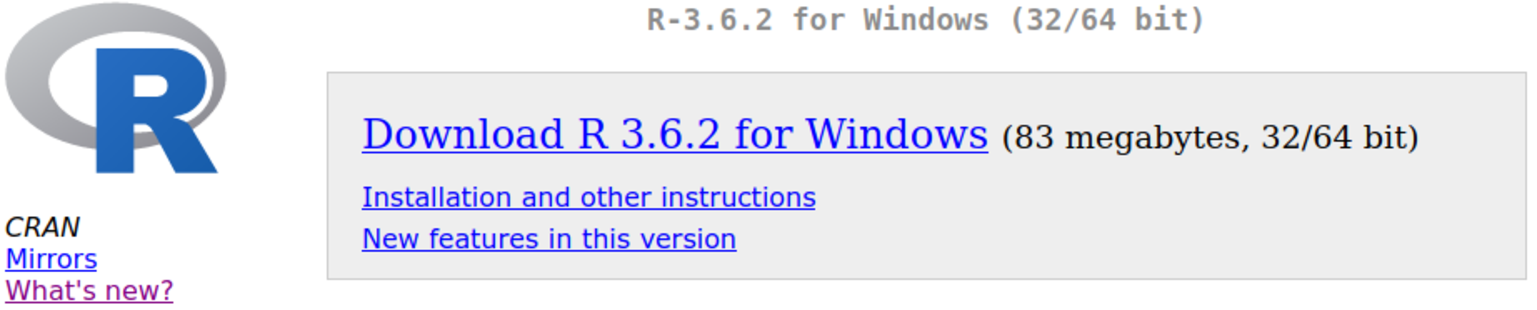
\includegraphics[width=\linewidth]{download-r}
    \label{fig:download-r}
  \end{figure}

\end{frame}

\subsection{\RStudio}

\myffr

  rstudio.com(\url{https://rstudio.com})から
  オープンソース版の\RStudio をダウンロードし,インストールする.

  \mybfr{手順}
    次のURLで「RStudio Desktop」の「DOWNLOAD」ボタンを押し,
    Windows版のインストーラをダウンロードし,実行する.
    \url{https://rstudio.com/products/rstudio/download}
  \mybto

  \vspace{1mm} 

  \begin{figure}[h]
    \centering
    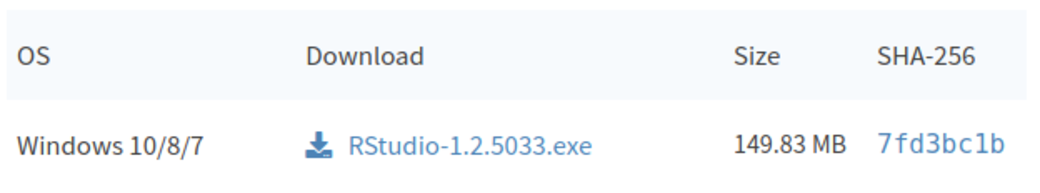
\includegraphics[width=\linewidth]{installer-rstudio}
    \label{fig:installer-rstudio}
  \end{figure}

\end{frame}

\myffr

\framesubtitle{CRANミラーサイト設定}

  デフォルトのCRANミラーサイトを国内サイト\\
  「41: Japan (Tokyo) [https]」に変更する.

  \mybfr{手順}
    コンソールで「chooseCRANmirror()」を入力し,\\
    「Selection:」のプロンプトが表示されたら「41」を入力する.
  \mybto

  \myefr{コンソール}
    \cs{chooseCRANmirror()}
    Secure CRAN mirrors\\
    \hspace{1mm}1: 0-Cloud [https]\\
    \hspace{1mm}2: Algeria [https]\\               
    \hspace{1mm}:\\               
    \textcolor{blue}{Selection: 41}
  \myeto

\end{frame}

\subsection{\R パッケージ}

\myffr

  \mybfr{手順}
    コンソールで「install.packages('***')」を入力する.\\
    ***には,インストールしたい\R パッケージ名が入る.
  \mybto

  \myefr{コンソール}
    \cs{install.packages('excel.link')}
  \myeto

  【注意】\\
  社内標準PCからは,この方法では\R パッケージを
  ダウンロードできない.
  対処方法としては,
  標準外PCで予めダウンロードし,
  \R インストールディレクトリ¥library内にある
  \R パッケージ,および,
  そのパッケージが依存するすべてのパッケージ
  (同一タイムスタンプで判別)を
  USBで標準PCのlibrary内にコピーする.

\end{frame}

\end{document}

